\documentclass[main.tex]{subfiles}
\begin{document}
\section{Transformers}

Next up in this section, the theory behind the transformer is introduced, including the main features comprising mainly of the concept of attention, positional encoding, and masking, and how they work in the form of an encoder-decoder architecture. Furthermore, an explanation of how the transformer can be suited for time series forecasting will be presented, including the modifications needed to make it work. And lastly the non-trivial parts of the implementation will be shown followed by the results of the model's performance on the power consumption data set.

\subsection{Theory}
The transformer is an encoder-decoder architecture, much like an auto-encoder, where the input is encoding with certain information, changing the structure of the input, and then decoded to change it back to something similar to the original structure. Among other things, what makes the transformer special is that it utilizes what is called \textit{attention}, which will be elaborated on below. A transformer can in theory be used to perform the same tasks as recurrent neural networks or convolutional neural networks, but by removing things like recurrent dependencies, it becomes possible to parallelize calculations. This together with attention, and adding elements such as positional encoding, masking among others, should set this type of model above others in these types of tasks, including time series forecasting, in both performance and precision \cite{Attention}. 

\subsubsection{Attention}
Attention works by mapping a set of queries and pairs of key-values to an output. The output is calculated by a weighted sum of the values, where the weights are assigned by the likeness of the key and the corresponding query \cite{Attention}. This score is calculated from the function:

$$\text{Attention}(Q,K,V) = \text{softmax}(\frac{QK^T}{\sqrt{d_k}})V$$

where \textit{Q}, \textit{K}, and \textit{V} are the queries, keys, and values respectively, with $d_k$ as the dimensions of the keys and queries, and values \textit{V} of dimension $d_v$. In the case of the attention layer in both the encoder and decoder, the query, key, and value is simply the normalized input which is returned from the positional encoding.\\
Also a \textit{Softmax} activation function is applied before multiplying with the values, which creates the weights by returning values between 0 and 1.\\
Now this above is what is called \textit{scaled dot product attention}, which only calculates attention for a single head, or layer. An evolution of this is \textit{multi-head attention}, and the difference here is that multi-head attention gathers more layers of the single-head attention layers, which in theory makes it able to focus on several time steps at once. This is done by applying the single-head attention function to \textit{n} different linear projections of the queries, keys, and values, which are concatenated, projected once again:

$$\text{MultiHead}(Q,K,V) = \text{Concat}(\text{head}_1,...,\text{head}_n)W^O$$

where each head is:

$$head_i = \text{Attention}(QW_i^Q,KW_i^K,VW_i^V)$$

And $W_i^Q \in \R^{d_{model}\times d_k}$,$W_i^K \in \R^{d_{model}\times d_k}$,$W_i^V \in \R^{d_{model} \times d_v}$, and $W^O \in \R^{hd_v \times d_{model}}$ are parameter-matrices for the projections \cite{Attention}. Both scaled dot-product attention and multi-head attention is visualized below.

\begin{figure}[H]
    \centering
    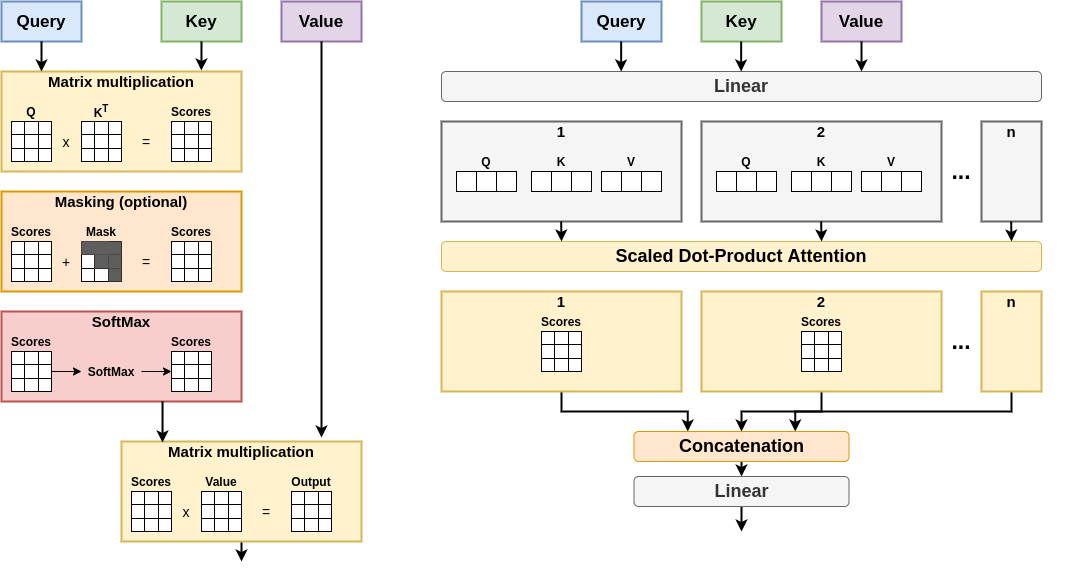
\includegraphics[width=0.9\textwidth]{Figures/Attention.png}
    \caption{(Left) Scaled Dot-Product Attention & (Right) Multi-Head Attention}
    \label{fig:Attention_figure}
\end{figure}

Another piece of the transformer is added to make sure that the decoder cannot look ahead and share information about future parts of the sequence, this is called masking.\\
Masking is implemented by creating a square matrix tensor of the same size as the attention scores, with zeros below the diagonal and $-\infty$ on the diagonal and above. The matrix or mask filter, is then added to the scores. Essentially acting as a weight matrix that weighs the later parts of the sequence lower, thereby hiding them from the model, making sure that it cannot simply look ahead in the sequence to predict the next entry \cite{HowToCodeTransformer}.

\subsubsection{Positional encoding and embedding}
Now the transformer model contains one more important element that differentiates it from other encoder-decoder models, which is essential as it injects information about the structure of the data sequence into the model. What is aptly called positional encoding is necessary as the encoder-decoder model does not contain the same recurrent structure such as an recurrent neural network or a convolutional neural network. \\
A token's position in a sequence is calculated and injected using the continuous functions \textit{sine} and \textit{cosine}, and given the position and dimension of the token:
$$PE_{(pos,2i)} = sin(pos(10000^{2i/d_{model}})$$
$$PE_{(pos,2i+1)} = cos(pos(10000^{2i/d_{model}})$$
With these functions, an encoding matrix is created with matching dimensions of the data, and then the two are added together to create the encoded data. An intuitive way to think about the encoding vector is as a number represented in binary, where each bit and their position gives the number. This is essentially the same case with this positional encoding, but instead of bits, floats are used, ranging in values between $2\pi$ and $10000 \cdot 2\pi$ on the sine and cosine wavelengths \cite{Positionalencoding}.\\
Normally, as the transformer from \cite{Attention} was originally devised for semantics analysis, the embedding layer was tasked with converting the language data to vectors, but as this project concerns time series data, in this case it is a just a linear transformation that maps the data's feature dimensions to the dimensions of the model.

\subsubsection{Normalization}
The normalization layer was implemented by the following function:
$$ \frac{\alpha_{d\_model} * (x - \mu_x)}{\sigma_{x}+\epsilon} + \beta$$
where $\alpha$ and  $\beta$ are vectors of size $d\_model$ containing ones and zeros respectively, and $\epsilon = 0.000001$, essentially computing the standard score by subtracting the mean of \textit{x} from \textit{x} and dividing by its standard deviation. 

\subsubsection{Feed Forward Neural Network}
Each layer contains a simple feed forward neural network, which in essence are two linear transformations with a \texttt{ReLU} activation between, followed by dropout. 

$$FFN(x) = \text{max}(0, xW_1 + b_1)W_2 + b_2 $$

These are present to act as a sort of convolution, where the projections are the same, from 128 dimensions to $4 \times 128$, and back again, different layers contains different parameters\cite{Attention}.\\
\\
With these elements, the structure of the transformer can now be visualized, and can be seen consisting of these different layers below. 

\begin{figure}[H]
    \centering
    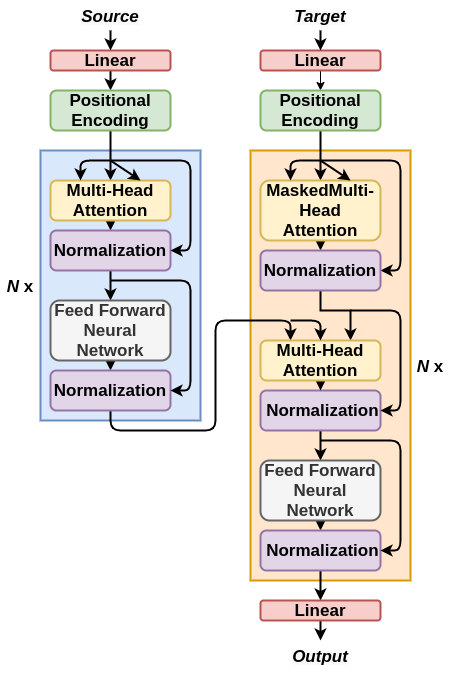
\includegraphics[width=0.6\textwidth]{Figures/transformerarchitecture.png}
    \caption{Transformer architecture}
    \label{fig:transformer_architecture}
\end{figure}

\subsection{Implementation}
For the implementation of the transformer, \texttt{pytorch}'s neural network library was used. The actual implementation of the different layers of the model simply follows all the layers presented above, instantiated in different classes to match their theoretic module counterpart.\\
\\
As for the LSTM model, the time series dataset was split into 60\%/20\%/20\% train/validation/testing. Furthermore, as the implementation uses \texttt{pytorch} dataloaders, the training was done in batch sizes of 36.\\
Furthermore, in terms of the actual hyperparameters of the transformer, following the recommendations of \cite{Attention}, the model was initialized with $d_{model} = 128$, 6 encoder/decoder layers, and 8 attention head layers. For the loss function, \textit{Mean Squared Error} (MSE) was used to measure the average of squares of errors between the predictions and the actual values. The optimizer that was used was Adam, which in very simple terms can be seen as a combination of \textit{RMSProb} and \textit{AdaGrad} \cite{kingma2017adam}, together with a very low learning rate of 0.0001. In terms of learning rate, this implementation deviated from the article \cite{Attention}, as they used a dynamic learning rate, and instead a choice was made here to simply use a static low learning rate, as the size of the problem in this case was much smaller.\\
With regards to the number of epochs, in the article\cite{Attention}, they run a great number of epochs, something that would not make sense here in terms of the size of the dataset and time spent, instead a form of adaptive stopping was run, where the validation loss was continuously evaluated, which was the case as for the training of the LSTM model, and which would stop training if the loss did not improve for a number of iterations, which was set to 10.

\subsection{Transformer results}
As mentioned, for the transformer, the focus was mainly on the multi-step predictions, as this is where the transformer in theory should separate itself from other "simpler" methods. 

\begin{figure}[H]
    \centering
    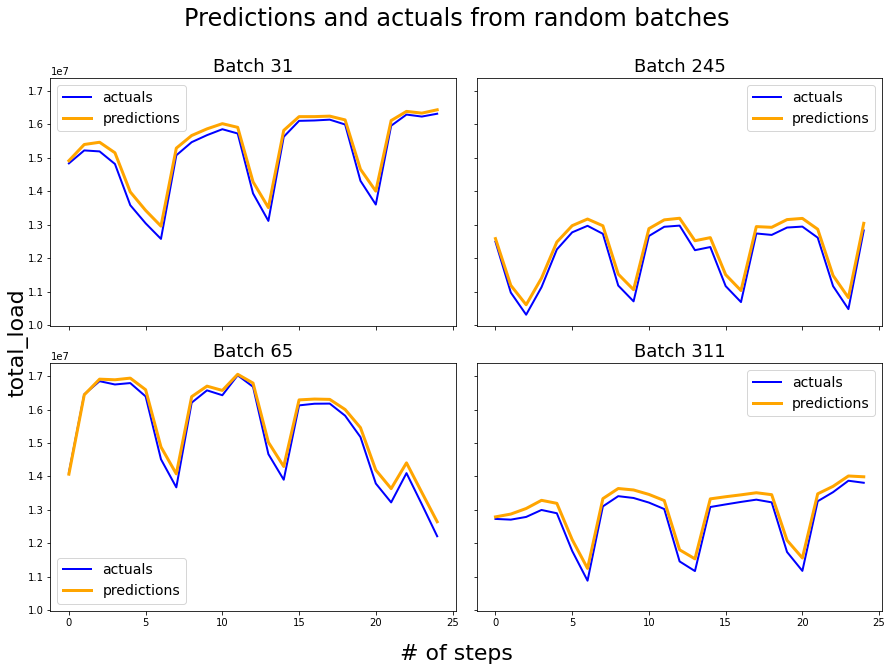
\includegraphics[width=0.8\textwidth]{TransformerPlots/transformerpredictionsgood.png}
    \caption{Transformer multi-step prediction of 25 days ahead, with look-back length of 50}
    \label{fig:transformer_pred1}
\end{figure}

What can clearly be seen from the different examples is that the transformer's predictions lie close to the actual data from the test set. The small differences that can be noticed however is that there are small gaps between the predictions and actual values, where it looks like the predictions lie above the actuals values. These are small differences, and one could expect that they could be mitigated with further tuning of the hyperparameters, something that was not a focus of this project. Whether not doing this was the right approach will be discussed later in the project. \\
Furthermore, as the model was trained to make predictions 25 days ahead from the last 50 days, there is a decent amount of data to make predictions from, which could also be the reason for these relatively good predictions.\\
The classification of "good predictions" is however not only based on visual inspection of the prediction plots, but also from the loss plot. What can be seen is that both the training loss and validation loss seem to converge towards almost zero loss after a relatively low number of epochs. It is interesting to note that the validation loss is lower than training loss, something that was generally the case throughout different runs.

\begin{figure}[H]
    \centering
    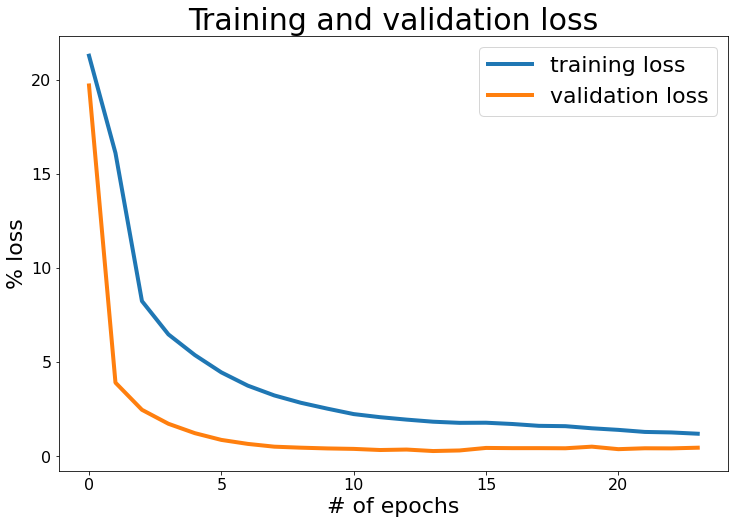
\includegraphics[width=0.6\textwidth]{TransformerPlots/transformerlossgood.png}
    \caption{Training and validation loss for the transformer with 25 day predictions}
    \label{fig:transformer_loss}
\end{figure}

Below, the capabilities of the transformer is emphasized by showing that the transformer does not need a very large amount of data to make its prediction with. As the plot shows, having the length of the look-back sequence the same size as the prediction still makes decent predictions, though the gaps between predicted and actual data become a bit larger.

\begin{figure}[H]
    \centering
    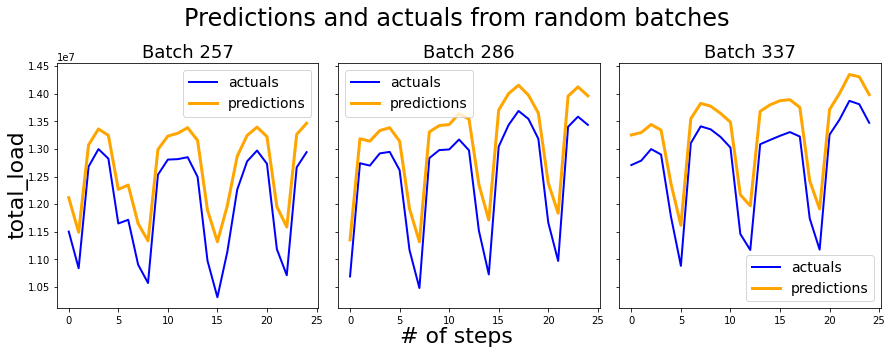
\includegraphics[width=0.9\textwidth]{TransformerPlots/transformerpredictionsnotasgood.png}
    \caption{Transformer multi-step prediction of 25 days, with look-back length of 25}
    \label{fig:transformer_pred_2}
\end{figure}

However, it does seem like the transformer is able to perform well even on longer predictions, as shown below, where really good predictions are shown on twice the number of steps, as long as it has enough data to make predictions from.

\begin{figure}[H]
\centering
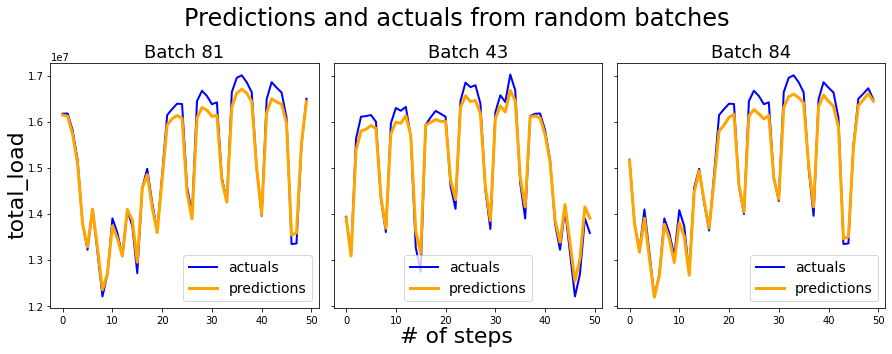
\includegraphics[width=0.9\textwidth]{TransformerPlots/transformerpredictionsgood3.png}
\caption{LSTM multi-step prediction of 50 days ahead, with look-back length of 50}
\label{fig:lstm_preds_1}
\end{figure}

Lastly, the average distance between the transformer predictions and actual values are plotted, in the same fashion as the LSTM model. This shows that the predictions are much more stable throughout the sequence, and though the difference in values are spiking, the predictions and actuals are much closer to each other overall, and the distance does not necessarily rise at the end of the prediction sequence.

\begin{figure}[H]
    \centering
    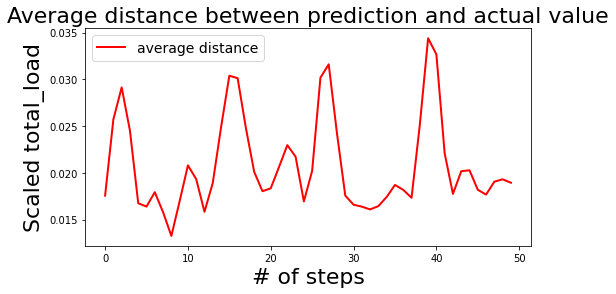
\includegraphics[width=0.7\textwidth]{TransformerPlots/avgerrortransformer.png}
    \caption{Average distance between predicted and actual values for the transformer}
    \label{fig:avgerrortransformer}
\end{figure}

\end{document}